%%%%%%%%%%%%%%%%%%%%%%%%%%%%%%%%%%%%%%%%%
% Simple Sectioned Essay Template
% LaTeX Template
%
% This template has been downloaded from:
% http://www.latextemplates.com
%
% Note:
% The \lipsum[#] commands throughout this template generate dummy text
% to fill the template out. These commands should all be removed when 
% writing essay content.
%
%%%%%%%%%%%%%%%%%%%%%%%%%%%%%%%%%%%%%%%%%

%----------------------------------------------------------------------------------------
%	PACKAGES AND OTHER DOCUMENT CONFIGURATIONS
%----------------------------------------------------------------------------------------

\documentclass[12pt]{article} % Default font size is 12pt, it can be changed here

\usepackage{geometry} % Required to change the page size to A4
\geometry{a4paper} % Set the page size to be A4 as opposed to the default US Letter

\usepackage{tabularx}
\usepackage[utf8]{inputenc}
\usepackage{csquotes}
\usepackage{listings}
\lstset{basicstyle=\ttfamily}

\usepackage{graphicx} % Required for including pictures

\usepackage{float} % Allows putting an [H] in \begin{figure} to specify the exact location of the figure
\usepackage{wrapfig} % Allows in-line images such as the example fish picture
\usepackage{soul}
\usepackage{lipsum} % Used for inserting dummy 'Lorem ipsum' text into the template

\usepackage{hyperref}

\usepackage[shortlabels]{enumitem}
                    
\usepackage{xcolor}


\linespread{1.2} % Line spacing

%\setlength\parindent{0pt} % Uncomment to remove all indentation from paragraphs

\graphicspath{{Pictures/}} % Specifies the directory where pictures are stored

\begin{document}
\setlist[enumerate, 1]{1\textsuperscript{o}}

%----------------------------------------------------------------------------------------
%	TITLE PAGE
%----------------------------------------------------------------------------------------

\begin{titlepage}

\newcommand{\HRule}{\rule{\linewidth}{0.5mm}} % Defines a new command for the horizontal lines, change thickness here

\center % Center everything on the page

\textsc{\Large Position Prediction Based on Movement Data}\\[0.5cm] % Major heading such as course name
\textsc{\large System Design Document}\\[0.5cm] % Minor heading such as course title

\vfill

\emph{Authors:}\\
Timo Jockers, Oliver Mänder, Benjamin Moser, \\
Manuel Prinz, Sebastian Strumbelj, Simon Suckut

\vfill % Fill the rest of the page with whitespace

\end{titlepage}

%----------------------------------------------------------------------------------------
%	TABLE OF CONTENTS
%----------------------------------------------------------------------------------------

\tableofcontents % Include a table of contents

\newpage % Begins the essay on a new page instead of on the same page as the table of contents 

%----------------------------------------------------------------------------------------
%	INTRODUCTION
%----------------------------------------------------------------------------------------

% Changelog 
\section{Änderungen}


\begin{tabular}{|c|c|p{10cm}|c|}
\hline
Version & Autor & Beschreibung & Datum \\ \hline\hline

%changelog content 
1.0 & ALL & Erstellen von SRS und SDD & 15.5.2018 \\\hline
	& BM  &	Klarstellung Begriff IDs  &	21.5.2018 \\\hline
	& BM  &	Neu: Abschnitte Erstinstallation, Erstausführung  &	22.5.2018 \\\hline
	& BM  &	Klarstellung Abschnitt 2.2  &	22.5.2018 \\\hline
	& BM  & Erweiterung Abschnitt 4.5   &   23.5.2018 \\\hline

\end{tabular}


{\small

\noindent
\\\\Legende: \\
SSJ = Sebastian Strumbelj \\
BM = Benjamin Moser \\
OM = Oliver Mänder \\
SS = Simon Suckut \\
TJ = Timo Jockers \\
ALL = SSJ, BM, OM, SS, TJ \\
}


%------------------------------------------------

\section{Einleitung} % Major section

%------------------------------------------------

\subsection{Zweck}
Das Erstellen einer App, um einem Ornithologen das Finden eines Vogels zu erleichtern, indem sie dessen zukünftige Position mit einem Vorhersagemodell abschätzt. 

%------------------------------------------------

\subsection{Design-Ziele}

Diese Dokumentation spezifiert alle Eigenschaften, die unsere App benötigt, um deren Zweck zu erfüllen. Um eine Vorhersage für Vögel zu treffen und dem Ornithologen bei seiner Suche zu unterstützen, sollte die App folgende Funktionen beinhalteten: 
\begin{itemize}
	\item Aufbereiten und Speichern der vorhandenden und für die Berechnung einer Vorhersage benötigten Tracking-Daten von Vögeln
	\item Berechnung einer Positionsvorhersage
	\item Visualisierung des Ergebnisses der Positionsvorhersage
	\item User-Interface zur Interaktion 
\end{itemize}
Der genaue Funktionsumfang ist im SRS definiert.



% This document fully specifies all traits relevant for the implementation of...

% The system does...

% The system does not...

\subsection{Definitionen und Abkürzungen}

	\paragraph{App, Applikation} Soweit nicht anders angemerkt wird hiermit die zu entwickelnde Android-Applikation bezeichnet.
	 \paragraph{Forscher} Personen, die wissenschaftlich das Verhalten von Vögeln untersuchen.
	 \paragraph{Mobile Daten} Ein Smartphone kann sich entweder über ein WiFi-Netzwerk oder über ein mobiles Datennetzwerk (3G, LTE, ...) mit dem Internet verbinden. 
	\paragraph{Vorhersage-Modell/Algorithmus} Die zur Berechnung einer Vorhersage verwendete Methodik. 
	\paragraph{API} \textit{Application Programming Interface}, hier insbesondere Schnittstellen mit Providern wie \textit{Movebank} oder \textit{Cesium}. 
	\paragraph{Outdoor-Modus, Normal-Modus} Die Applikation verfügt über zwei verschiedene Funktionsmodi. Einer davon ist der sog. Outdoor-Modus.
	\paragraph{Cesium} ...ist eine Javascript-Bibliothek für die Arbeit mit dreidimensionalen Kartendaten.
	\paragraph{Offline-Karten} ...ist ein 2D-Karten-Provider der Kartendaten liefert, wenn keine Internetverbindung besteht.
	\paragraph{StudyID, VogelID} Eindeutige Identifikatoren einer Studie bzw. eines einzelnen Vogels in der \textit{Movebank}-Datenbank.  
	\paragraph{SRS} Software Requirements Document



\subsection{Referenzen}
\begin{itemize}
	\item SRS
	\item Treffen mit den Betreuern
	\item Treffen mit einem Forscher
	\item \href{https://git.uni-konstanz.de/kn/swp2018/group12/tree/master/Dokumentation/Lizenzen}{Notizen zu Recherche über Nutzungsbedingungen und Lizenzen von Systemkomponenten}.
\end{itemize}


\subsection{Überblick}

Der erste Teil legt grundlegende Ideen und Definitionen der App fest. Der zweite Teil beschäftigt sich mit bereits existierenden und ähnlichen Systemen. Der dritte Teil liefert eine Beschreibung für die für unsere App genutzte Architektur.  





\section{Aktuelle Architektur}

\enquote{Animal Tracker} ist bereits eine App, welche Trackingdaten von Vögeln visualisiert. Allerdings berechnet diese keine Vorhersagen für die Zukunft und fokussiert sich dementsprechened nur auf die Darstellung vergangener Daten. Interne Architekturen dieser App sind allerdings nur gering bekannt.


\section{Vorgeschlagene Architektur}



\subsection{Teilsysteme und Hardware-Software-Zuordnung}

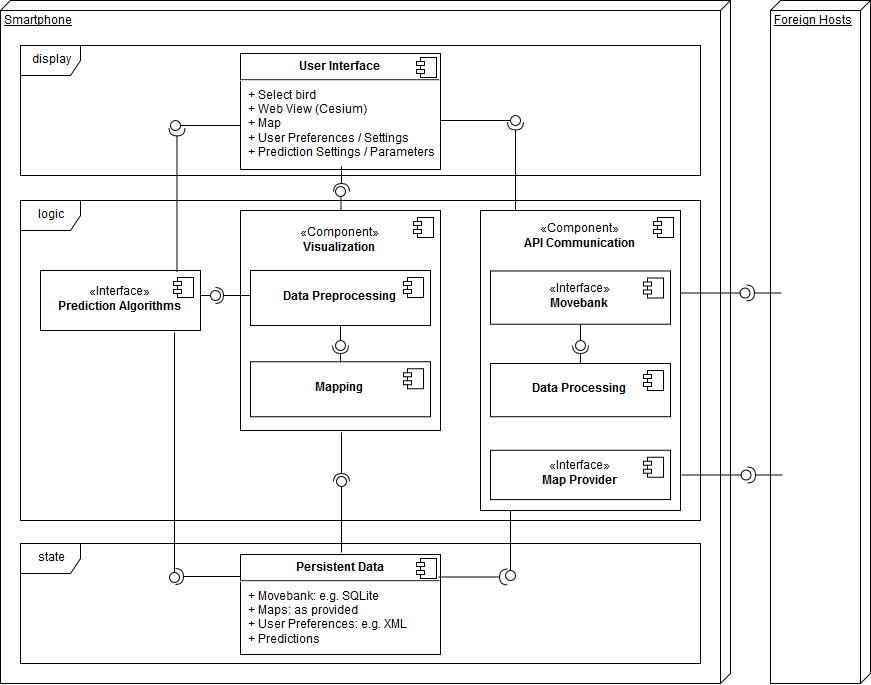
\includegraphics[width = \textwidth]{Diagramme/ComponentDiagram.png}

\vspace{1em}

Das SRS verlangt ein modulares Softwaresystem. Die Subsysteme sind dazu in einer dreischichtigen Architektur (State, Logic, Display) eingebettet. Die Benutzeroberfläche stellt verschiedene \textit{Activities} zur Verfügung, in der zum einen Nutzereingaben getätigt werden können (Nutzerdaten/-einstellugen, Auswahl des Vogels und Parametereinstellungen für den Vorhersagealgorithmus) und zum anderen die Ergebnisse der Berechnung visualisiert werden (als Kartenansicht und/oder Cesium-WebView).

Abhängig von dem gewählten Vogel bezieht das System Daten von der \textit{Movebank}-API, verarbeitet sie so, dass sie für eine Vorhersage verwendet werden können und speichert sie in der lokalen Datenbank, falls sie dort noch nicht vorhanden sind. Ebenso werden benötigte Kartendaten von einem geeigneten Anbieter abgerufen und lokal gespeichert. Die gespeicherten Daten werden für die Vorhersage verwendet, deren Ergebnisse wiederum lokal gespeichert werden. Diese werden für die Visualisierung aufbereitet und auf der Karte bzw. in Cesium dargestellt.

\subsection{Management von persistenten Daten}

Um Daten nach dem Schließen der Applikation zu behalten, die Menge des Datenvolumens für Anfragen an die Movebank zu reduzieren und um Daten leichter verwalten zu können verfügt die Applikation über eine Schnittstelle zum Parsen und Speichern von XML-Dateien und eine SQLite-Datenbank. Außerdem werden Karten für den Outdoor-Modus lokal gespeichert.

\begin{itemize}
	\item \textit{SQLite-Datenbank}: In dieser Datenbank werden Daten von der Movebank lokal zwischen gespeichert. Dadurch wird die Menge an Anfragen an die Movebank so gering wie möglich gehalten, die Menge des verbrauchten Datenvolumens reduziert und die Daten werden leichter zu verwalten.
	
	\item \textit{XML-Parser}: In der Applikation getätigte Einstellungen werden persistent in einer XML-Datei gespeichert.
	
	\item \textit{Offline-Karten}: Karten-Daten werden in dem vom Kartenanbieter verwendeten Format lokal zwischengespeichert.
	
	
\end{itemize}

% -------------------------------------------------------------------


\subsection{Sicherheit}
Mit einem Benutzernamen und einem Passwort kann der Zugriff für die Movebank-Daten erweitert werden. Es gibt aber keinen erweiteren Zugriff (z.B. auf die Verwaltung) der App. 


% Übersetzung?
\subsection{Global Software Control}

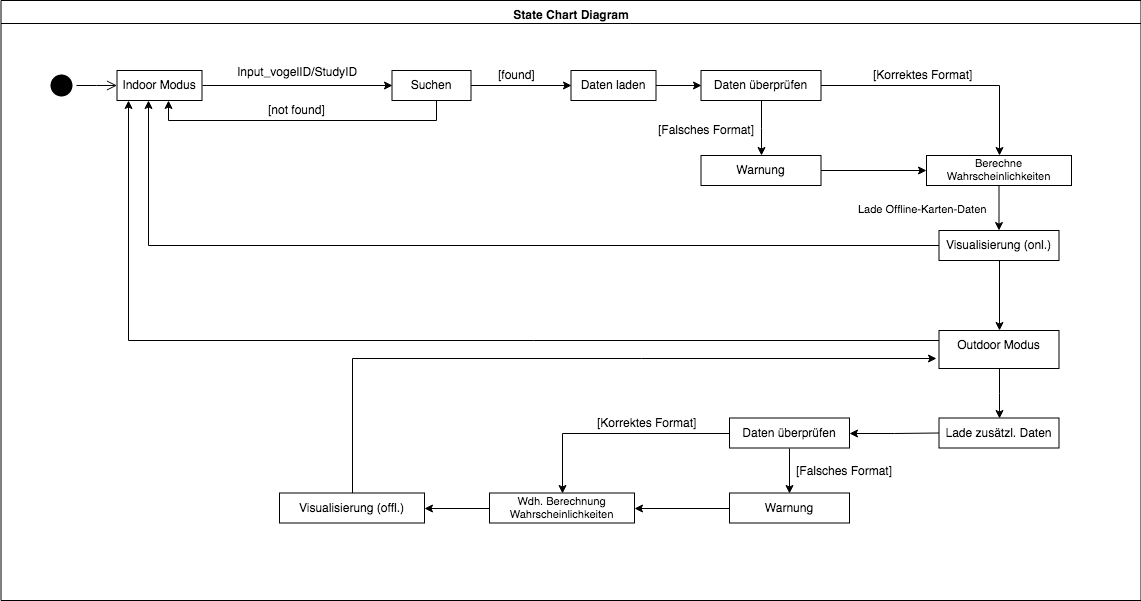
\includegraphics[width = \textwidth]{Diagramme/state_diagram.png}

\vspace{1em}

Das Global-Software-Control-Diagram beschreibt das allgemeine Verhalten der App. Es besteht aus dem allgemeinen Ablauf der App im Indoor- (obere Hälfte) und Outdoormodus (untere Hälfte). 

Zu Beginn befinden wir uns im Indoor-Modus und können nun mit der VogelID und StudyID nach einem Vogel suchen. Ist der Vogel nicht verfügbar, so haben wir keine Möglichkeit, weiter zu machen und beginnen von vorne. Ist er vorhanden, so laden wir dessen Daten. Anschließend werden diese geprüft bzw. geparst. Im Fall, dass die Daten formal falsch sind (siehe SRS für die Definition von formal falsch), werden diese trotzdem zur Berechnung benutzt. Allerdings wird eine Warnung über die Qualität der Daten erscheinen. Nach dem Berechnen der Wahrscheinlichkeiten, werden die Kartendaten und weitere Daten für die Visualisierung heruntergeladen, um diese auch ohne Internetverbindung visualisieren zu können. Solange wir uns aber im Indoor-Modus befinden, können diese mit Cesium visualisiert werden. Sollen andere Vögel untersucht werden, so kann die Suche von vorne beginnen.

Geht der Forscher nun in das Feld, schaltet er in den Outdoor-Modus. Der Ablauf ist nun ähnlich wie im Indoor-Modus. Es können zusätzliche oder neue Daten des Vogels über die mobile Datenverbindung geladen werden. Sie fließen in die erneute Wahrscheinlichkeitsberechnung ein und aktualisieren die Visualisierung, die nun allerdings mit einem Offline-Karten-Provider dargestellt wird. 
% • How will control signals be used?
% • How do the subsystems communicate? --> interface descriptions?
% • How do the subsystems synchronize? --> statechart diagram? Concurrency

\subsubsection{Interfaces}
\label{sec:interfaces}
\begin{itemize}
	\item Tracking-Daten werden von der \textit{Movebank}-Datenbank bezogen. Hierfür stellt diese eine Web-API bereit. Es sind verschiedene Endpunkt verfügbar:
	\begin{itemize} 
	 	 \item  \lstinline$/movebank/service/direct-read$ 
	 	 \item \lstinline$/movebank/service/public$
	 	 \item \lstinline$/movebank/servie/json-auth$
	\end{itemize} 
	Es wird von der Applikation ausschließlich der Endpunkt \lstinline$direct-read$ verwendet.
	% \item Daten werden über ein Movebank-Inteface geladen und verarbeitet. 
	\item Daten werden mittels einem Cesium-Interface im Indoor-Modus visualisiert.
	\item Daten werden mittels einem Open-Street-Map-Interface im Outdoor-Modus visualisiert.
\end{itemize}
% ----

% Übersetzung?
\subsection{Boundary Conditions}
In diesem Abschnitt werden Randfälle beschrieben, die in der Kommunikation mit Schnittstellen auftreten können sowie desweiteren wie diese behandelt werden.
\subsubsection{Anfrage}
In Diagramm \ref{seqDiagAnfrage} wird der Ablauf einer Datenanfrage von der \textit{Movebank}-API sowie darauffolgend vom Provider der 2D-Karten dargestellt.
\begin{figure}[h]
		% <left> <lower> <right> <upper>
		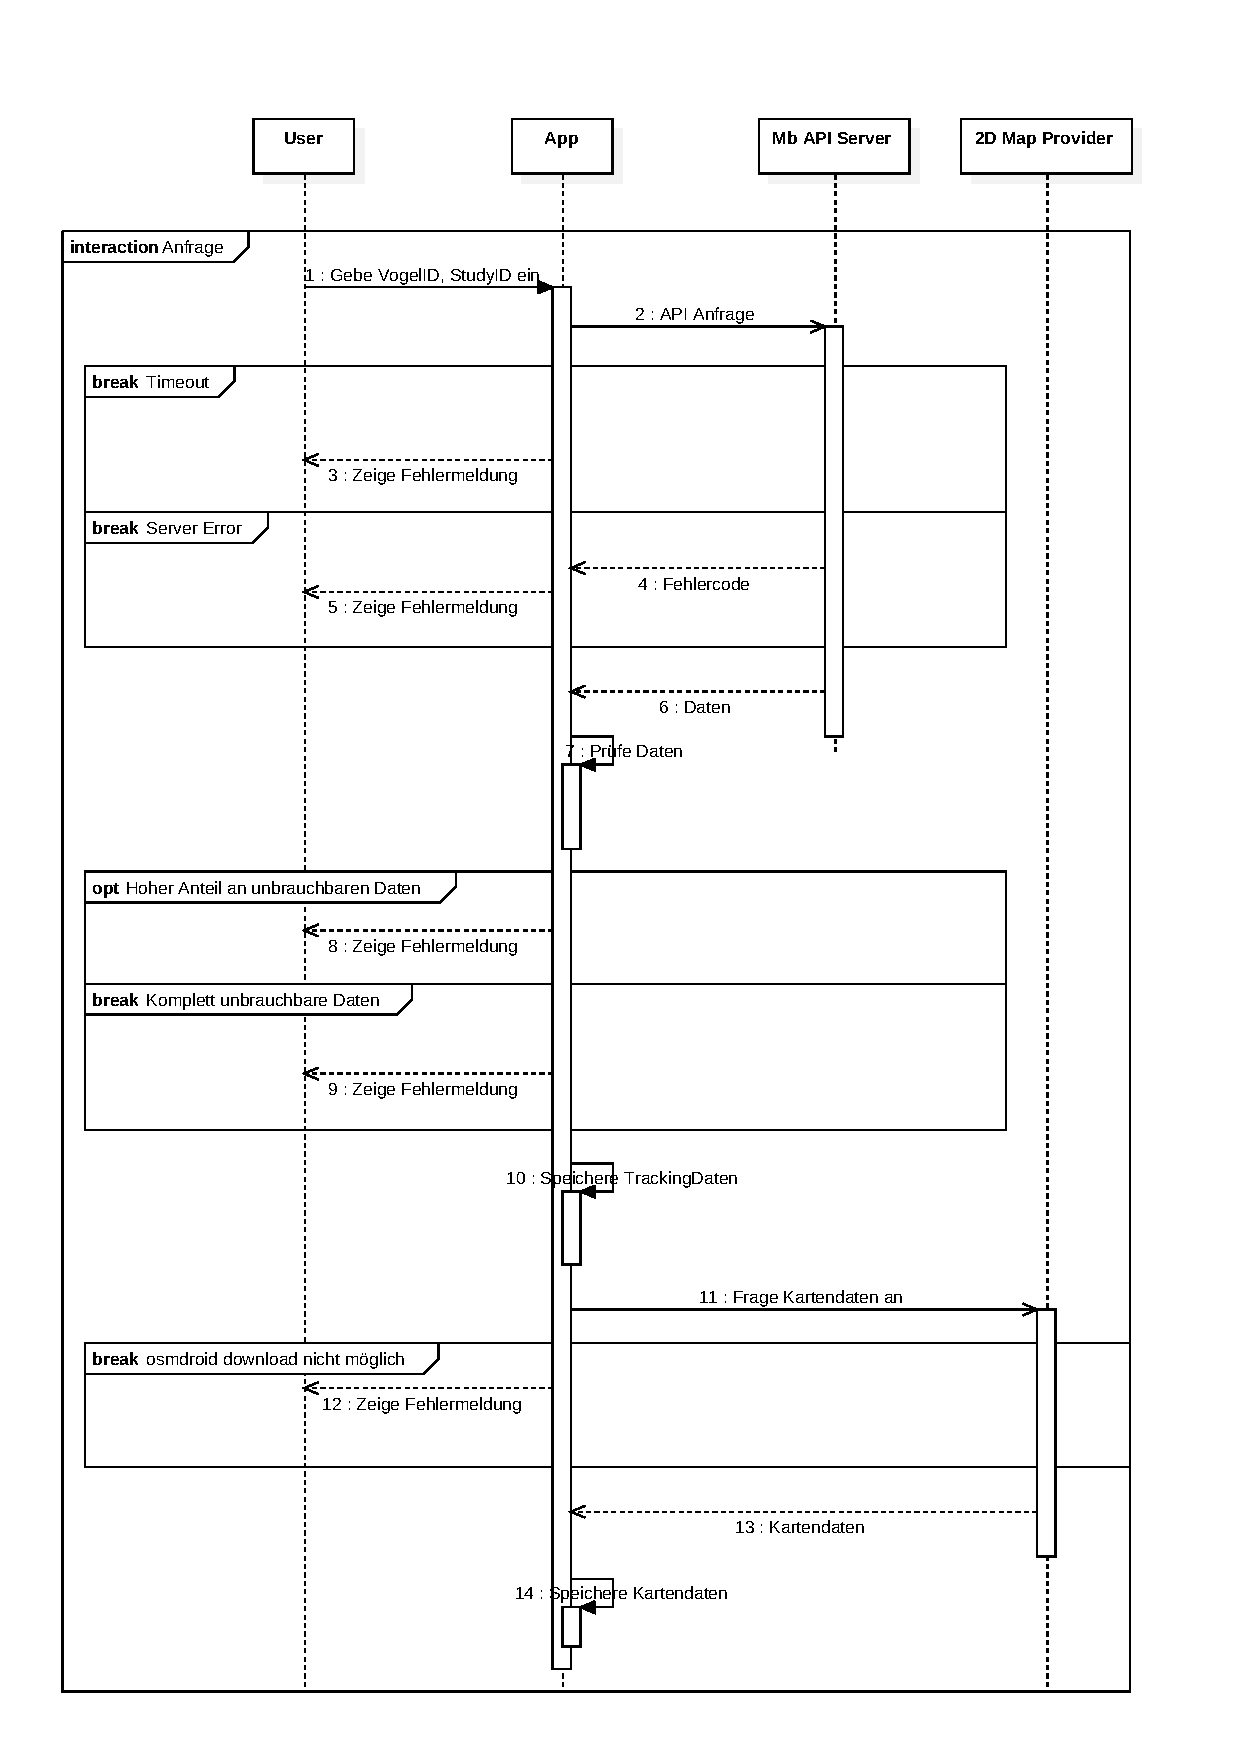
\includegraphics[height=0.95\textheight,trim={0 1cm 5cm 2cm}]{Diagramme/SeqDiag-Abfrage.pdf}
		\caption{Anfrage}
		\label{seqDiagAnfrage}
	\hspace*{\fill}
\end{figure}

% \begin{enumerate}[label={\arabic*.}]
% \item Der Nutzer startet die App.
% \item Der Nutzer wird dazu aufgefordert, VogelID und StudyID einzugeben, um die Daten für einen bestimmten Vogel abzufragen.
% \item Die App sendet eine Anfrage an die Movebank, um die Daten für den vom Nutzer gewollten Vogel zu erhalten.
% \item Wenn der Movebank Server nicht erreichbar ist, wird dem Nutzer eine Meldung darüber angezeigt und keine Vorhersage berechnet.
% \item Die App sendet die Accountdaten aus den Einstellungen zur Movebank.
% \item Wenn die Accountdaten für die Movebank nicht gültig sind, wird dem Nutzer eine Meldung darüber angezeigt und keine Vorhersage berechnet.
% \item Wenn die eingegebenen IDs nicht gültig sind, wird dem Nutzer eine Meldung darüber angezeigt und keine Vorhersage berechnet.
% \item Sind die IDs gültig, so werden die Daten aus der Movebank heruntergeladen.
% \item Wenn während dem Download die Interverbindung abbricht, wechselt die App in den Outdoor-Modus und setzt den Nutzer darüber in Kenntnis.
% \item Bleibt die Internetverbindung bestehen, werden die Daten vollständig aus dem Internet heruntergeladen und die App berechnet eine Vorhersage.
% \end{enumerate}


\paragraph{Erläuterungen zu Segment "Server Error"} 

Hier können verschiedene Szenarien
auftreten, die aber alle hinsichtlich des Informationsaustausches gleichförmig sind.
\begin{itemize} 
 	 \item HTTP-Status ist \lstinline$500 Internal Server Error$ -- Der Nutzer wird informiert, dass der Server momentan nicht erreichbar ist.
 	 \item HTTP-Status ist \lstinline$401 Unauthorized$: Keine Zugangsdaten in Anfrage vorhanden. In diesem Fall wird dem Nutzer ein Hinweis angezeigt mit der Aufforderung, seine Zugangsdaten in den Einstellungen der App einzutragen. 
 	 \item HTTP-Status ist \lstinline$200 OK$
 	 \begin{itemize} 
 	   	 \item Response Body ist \lstinline$<p>No data are available for download.</p>$. -- Informiere Nutzer, dass keine Daten vorhanden sind.
 	   	 \item Response-Header ist \lstinline$accept-license: true$ -- In diesem Fall hat der Nutzer noch nicht die Nutzungsvereinbarung akzeptiert. Dies wird dem Nutzer über einen Hinweis mitgeteilt. Wie im SRS spezifiziert wird hier davon ausgegangen, dass dies durch den Nutzer gewährleistet wird.
 	   	 \item Response-Body beginnt mit \\ \lstinline$Specify one of the following entity types: deployment, event, ...$ In diesem Fall konnten die Anfrageparameter nicht von der API interpretiert werden. Zeige Hinweis an den Nutzer, dass die Anfrage nicht möglich war. 
 	  \end{itemize}  
 	  \item HTTP-Status ist irgendein anderer Fall der hier noch nicht aufgeführt wurde -- Dem Nutzer wird ein Hinweis angezeigt, dass die Anfrage nicht erfolgreich durchgeführt werden konnte.
\end{itemize} 

In jedem Fall wechselt die App nach Anzeigen des Hinweises in den Zustand vor der getätigten Anfrage.


\subsubsection{Besondere Abläufe bei Einrichtung}

\paragraph{Bei Erstinstallation:} Bei Erstinstallation der Applikation
müssen keine besonderen Prozeduren ausgeführt werden. 

\paragraph{Bei Erstausführung:} Bei Erstausführung müssen keine besonderen
Prozeduren ausgeführt werden. Bei Erstausführung werden noch keine Movebank-Zugangsdaten in den App-Einstellungen eingetragen sein. Bei Anfrage von Daten,
die Zugangsdaten erfordern verfährt das System wie im SRS im Abschnitt 7.1 (Anwendungsfälle) spezifiziert. 

% Startup behaviour (What happens, when we start the system?)
% • Shutdown behaviour (What happens, when we stop the system?)
% • Failure behaviour (What happens, when the system
% missbehaves? Which kind of failures can you imagine? What
% does the system need to do then?)



% \section{Anhänge}

% \subsection{Geänderte Anforderungen}

% % List changed requirements in old and new form.

%----------------------------------------------------------------------------------------

\end{document}